\section{Офисное ПО}
Компания Microsoft открыла формат doc (стандарт по которому он создается) только в 2000 г. До этого разработчикам приходилось методом обратного инженеринга вручную раскрывать этот стандарт. Это характеризует формат doc не в лучшую сторону -- не все имели доступ (Microsoft Word -- платное ПО) и формат проверен малым количеством людей. До сих пор существует много ошибок, которые исправлены только в docx.
\\Форматы odt и docx используют XML. Технология XML открыта -- любой может посмотреть, найти ошибки, предложить исправление. Чтобы убедиться, что odt и docx используют XML, есть простой способ: создайте docx или odt документ, смените расширение на zip и распакуйте. Можно увидеть, что в основном все файлы имеют расширение xml.
\\Нормальная криптография появилась только в docx. В формате doc ничего нельзя было шифровать. Только сторонними приложениями.
\\
\begin{center}
Стоимость продуктов Microsoft Office
\end{center}
\begin{itemize}
  \item Для дома и учебы (Word, Excel, PowerPoint, OneNote) $\approx$ 3000р.
  \item Для дома и бизнеса (Word, Excel, PowerPoint, OneNote, Outlook) $\approx$ 10000р.
  \item Профессиональный (Word, Excel, PowerPoint, OneNote, Outlook, Access, Publisher) $\approx$ 20000р.
\end{itemize}
LibreOffice, OpenOffice, Calligra Suite = 0р.
\\
\\В 2010 году был принят ГОСТ Р ИСО/МЭК 26300--2010, обязывающий госучреждения перейти на бесплатный формат документов (Open Document Format -- ODF). Но это вовсе не означает, что будет использоваться LibreOffice и OpenOffice. В последних версиях Microsoft Office есть поддержка этого формата.
\begin{figure}
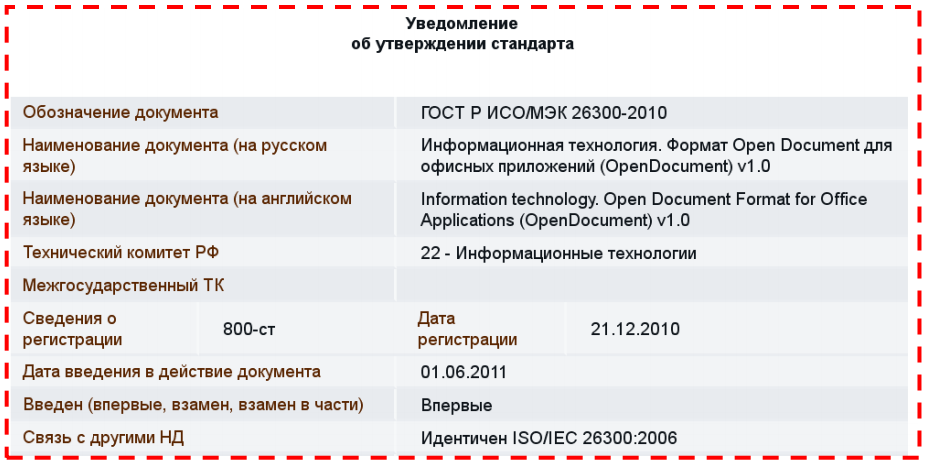
\includegraphics[width=\textwidth]{8_1}
\caption{ГОСТ Р ИСО/МЭК 26300--2010}
\end{figure}
\begin{center}
\emph{ ODF}
\end{center}

\begin{itemize}
  \item Распоряжение Правительства Российской Федерации от 17 декабря 2010 г. №2299--р "О плане перехода федеральных органов исполнительной власти и федеральных бюджетных учреждений на использование свободного программного обеспечения (2011 -- 2015 годы)"
  \item OpenDocument это единственный формат электронной документации, который реализован несколькими производителями ПО и утвержден ISO в качестве международного стандарта.
  \item Абсолютно любой производитель ПО может использовать формат OpenDocument при разработке своего собственного редактора
электронных документов.
  \item Продолжительный цикл существования формата OpenDocument обеспечен стабильностью спецификации.
  \item Открытость формата OpenDocument способствует росту его популярности среди производителей ПО, в числе которых есть производители бесплатных и открытых продуктов. 
  \item Открытость формата OpenDocument позволяет пользователю быть свободным при выборе программного обеспечения, не зависеть от конкретного поставщика ПО и его маркетинговой политики.
  \item Исчезает угроза утери информации из--за изменения закрытых форматов
\end{itemize}
Недостатки ODF:
\begin{itemize}
  \item Спецификация  стандарта не определяет некоторые  элементы офисного программного обеспечения. По этой причине каждый разработчик может реализовывать эти элементы по--своему, что может привести к несовместимости соответствующих файлов.
  \item Новые версии стандарта выходят спустя большие промежутки времени. По этой причине недостатки текущей версии стандарта находят отражения в большем числе его реализаций.   
  \item Некоторые специалисты считают, что Microsoft, с целью вернуть монопольное положение на рынке, может создать свою реализацию формата OpenDocument с закрытым кодом,  которая  станет неоспоримым лидером среди реализаций OpenDocument. Далее, по мнению этих специалистов,  на эту реализацию перейдёт основная масса пользователей и государственных органов – после этого Microsoft внесёт изменения в очередную версию продукта, благодаря которым файлы, созданные в этой программе перестанут быть совместимыми с форматом OpenDocument.
\end{itemize}
Работа по стандартизации OpenDocument включает в себя:
\begin{itemize}
  \item \textbf{OpenDocument 1.0} (второе издание) OASIS (англ. Organization for the Advancement of Structured Information Standards) соответствует опубликованному стандарту ISO/IEC 26300:2006. Содержание ISO/IEC 26300 и OASIS OpenDocument v1.0 2--е издание идентичны. Оно включает в себя изменения, внесенные редакционным решением JTC1 ( англ. Joint Technical Committee 1) и доступно в ODF, HTML и PDF форматах.
  \item \textbf{OpenDocument 1.1} включает дополнительные возможности для решения проблем доступности. Он был утвержден в качестве стандарта OASIS на 2007--02--01 после голосования, опубликованного 2007--01--16. Публичное заявление было сделано 2007--02--13. Эта версия не была изначально представлена ISO / IEC, потому что это считается незначительным обновлением только ODF 1.0, и OASIS работали уже на ODF 1.2 в тот момент, когда ODF 1.1 была утверждена. Однако позднее было представлено ISO / IEC (по состоянию на март 2011 года, он был в "стадии запроса'' как проект поправки 1-- ISO/IEC 26300:2006/DAM 1) и опубликовано в марте 2012 года, как ISO / IEC 26300: 2006 / Amd 1: 2012 -- Open Document Format for Office Applications (OpenDocument) v1.1.
  \item  \textbf{OpenDocument 1.2} был утвержден в качестве спецификации OASIS на 2011--03--17 и в качестве стандарта OASIS на 2011--09--29. Он включает в себя дополнительные функции доступности, RDF--метаданные, электронную таблицу спецификаций формул, основанную на OpenFormula, поддержку цифровых подписей и некоторые особенности, предложенные общественностью. В октябре 2011 года ожидалось, что технический комитет OASIS ODF "скоро начнет процесс предоставления ODF 1.2 в ISO / IEC JTC 1 ". В мае 2012 года преставители ISO / IEC JTC 1 / SC 34 / WG 6 сообщили, что после некоторой задержки, процесс подготовки ODF 1.2 для представления JTC 1 для PAS транспозиции ведется в настоящее время.
\end{itemize} 
\subsection{Наиболее популярные офисные пакеты}

\begin{table}[!h]
 \begin{tabular}{|l|c|c|c|}
\hline
Название  &   & Примерная  &  \\
офисного  & Особенности &  стоимость на  & Исходный\\
пакета & & 2017 год, руб. &  код  \\
\hline
Google Docs, & Узкая ориентация & &\\
Яндекс.Диск, & на публичные &  бесплатно & закрытый \\
Облако Mail.ru  & облачные решения & & \\
\hline
 &  Имеет наиболее богатый &  &  \\
 Microsoft Office &  функционал, захватил  &  5000--35000&  закрытый\\
 & > 90\% desktop--установок  & & \\
\hline
LibreOffice,& Слабая поддержка & & \\
OpenOffice, & одновременного &  бесплатно & открытый \\
Calligra Suite & редактирования & & \\
\hline
 & Узкая ориентация на & & \\
iWork & на технику фирмы Apple &  бесплатно & закрытый \\
\hline
 & Интерфейс идентичен & 5000 & \\
WPS Office & Microsoft Office &  (0 с рекламой) & закрытый \\
\hline
WordPerfect & Узкая ориентация на рынок&  & \\
Office &  персональных компьютеров & 5000--25000 & закрытый \\

\hline
OnlyOffice & Приоритетная ориентация  & & \\
Feng Office & на частные и публичные &  бесплатно & открытый \\
  & офисные решения & & \\
\hline
 \end{tabular}
\caption{Наиболее популярные офисные пакеты}
\end{table}
В таблице рассмотрены не все 30 разновидностей офисных пакетов, а наиболее популярные. Популярность оценена  с помощью  сайта Trends Google, где отслеживается частота запросов пользователей со всего мира.
В таблице указаны офисные пакеты по убыванию популярности.
\subsection{Сравнение возможностей OO и MS Office}
\begin{table}[!h]
 \begin{tabular}{|l|c|c|}
 \hline
 Свойства & Open Office Calc & Microsoft Excel \\
 \hline
 Размерность & 1 024 $\times$ 1 048 576  & 16 384 $\times$ 1 048 576 \\
 \hline
 Кол--во цветов & 104 & 16 777 216 \\
  \hline
 Работа с & от 1 января 0001 г. & от 1 января 1900 г. \\
 датами & до 31 декабря 9999г. & до 31 декабря 9999г. \\
 \hline
 Поддержка  & met, pbm, pgm, ppm,  & cdr, emz, mix, pcz, \\
 графических & psd, ras, sbm, sgg, &  wmz, wpg, fpx,  \\
 форматов & svg, xpm, xbm &  drw \\
 \hline
 & Работа с MySQL. Макросы & Продвинутые сводные  \\
 Прочее & на разных языках & таблицы и условное \\
 & (Python, JavaScript) & форматирование  \\
  \hline
 \end{tabular}

\end{table}
\begin{center}
  \emph{Open Office Writer}
\end{center}
\begin{itemize}
  \item Частые обновления
  \item Независимые стили страниц в одном документе
  \item Автоматическое создание указателя формул
  \item Продвинутая навигация (по ссылкам, разделам, примечаниям, изображениям)
  \item Проверка орфографии любого количества языков в одном документе
  \item Вложенные, скрытые, защищенные паролем индивидуально оформленные разделы
  \item Перекрестные вычисления между разными таблицами в одном документе
  \item Несколько оглавлений в одном документе.
  \item Автоматизированное перемещение элементов оглавления и списков с подпунктами.
\end{itemize}
\begin{center}
  \emph{Microsoft Word}
\end{center}
\begin{itemize}
  \item Встроенные средства для продвинутой проверки грамматики русского языка
  \item Распознавание голоса и рукописного ввода
  \item Подробная справочная система с примерами
  \item Широкая распространенность
\end{itemize}
Если сравнивать \emph{производительность} OpenOffice Writer и Microsoft Word, то Writer уступает приблизительно в два раза.
\\Если сравнивать \emph{безопасность} OpenOffice и Microsoft Office, то Microsoft намного надежнее, чем OpenOffice (MS Office 2010: 17 крахов и 0 потенциальных уязвимостей, В OpenOffice 3.2.1: 163 краха и 18 потенциальных уязвимостей). Одна из причин -- разработкой свободного ПО занимаются любители.
\subsection{Концепция стилей и шаблонов}
\begin{itemize}
  \item 1--я ошибка -- форматирование вручную без стилей.
  \item 2--я ошибка -- создание оформления вместо создания структуры.
  \item При подготовке документа главное то, чем текст является. А как он выглядит -- вторично.
  \item Забыть про "размер шрифта 14pt"\, "гарнитура Times New Roman"\, "расположение по центру" и так далее.
  \item Помнить только стили: "Заголовок"\, "Заголовок $n$--ого уровня"\, "основной текст", и так далее.
  \item Создание нового документа начинается с продумывания структуры документа и создания системы стилей.
  \item Как будет выглядеть конечный документ, (шрифты, гарнитура, и так далее) решается, когда документ уже готов, путем изменения соответствующего стиля.
\end{itemize}
\subsection{Панграммы}
\textbf{Панграмма} (греч. "\emph{все буквы}") или разнобуквица -- текст, использующий все или почти все буквы алфавита.
Используется для:
\begin{itemize}
  \item Демонстрация шрифтов.
  \item Проверки передачи текста по линиям связи.
  \item Тестирование печатающих устройств.
\end{itemize}
\begin{description}
  \item[Microsoft] Съешь [же] ещё этих мягких французских булок, да выпей чаю.
  \item[KDE] Широкая электрификация южных губерний даст мощный толчок подъёму сельского хозяйства.
  \item[Gnome] В чащах юга жил бы цитрус? Да, но фальшивый экземпляр!
\end{description}
\subsection{Автозаполнение}
\textbf{Lorem ipsum} -- название классического текста--"рыбы".
\\\textbf{"Рыба"} -- слово из жаргона дизайнеров, обозначает условный, зачастую бессмысленный текст, вставляемый в макет страницы.
\\
\\Lorem ipsum представляет собой искаженный отрывок из философского трактата Цицерона "О пределах добра и зла", написанного в 45 году до нашей эры на латинском языке. Впервые этот текст был применен для набора шрифтовых образцов неизвестным печатником в XVI веке.
\\
$$=rand(m, n)$$
Где:
\\$m$ – количество абзацев;
\\$n$ – количество предложений в каждом абзаце;
\\Так же
$$=lorem(m, n)$$
\subsection{Табличный процессор}
Табличный процессор офисного ПО обладает многими очень полезными функциями, которые заметно упрощают работу с электронными таблицами:
\begin{itemize}
  \item Запрет на ввод некорректных значений в ячейку.
  \item Условное форматирование.
  \item Фильтры для заполненных таблиц.
  \item Расчет доверительного интервала.
  \item Подбор параметра (решение уравнений, имеющих только единственное решение).
\end{itemize}
\section{Вспомогательное ПО для программирования}
\begin{itemize}
  \item Автоматическое создание документации для программы (doxygen).
  \item Контроль версий (SVN, Git, Mercurial).
  \item Управления жизненным циклом найденных ошибок (bug tracking system).
  \item Автоматизированное тестирование кода и функциональности.
\end{itemize}
\subsection{Автоматизированное создание документации}
Самая известная система для автоматизации создания документации программного обеспечения на С/С++ -- это \emph{doxygen}. Используется в KDE, IBM, AbiWord, Adobe, DC++, Qt, \dots
\\При работе с Doxygen размечается код (в комментариях появляется собственный синтаксис, в результате чего комментарии преобразовываются в документацию).
\\
\\Такие программы значительно облегчают работу: не нужно отдельно создавать документацию. Более того, в комментариях все подробно описано и любой программист сможет разобраться в программе.
\subsection{Системы управления (контроля) версиями}
\begin{itemize}
  \item \textbf{Клиент--серверные (централизованные)}: CVS, Subversion, Microsoft SourceSafe, Perforce, VSS
  \item \textbf{Распределенные:} Mercurial, git
  \end{itemize}
\emph{Принцип работы}: пометка версий, которые отдаются пользователю, выкладываются на сайт (release версий) и версий для разработчиков, в которую возможно внести изменения (которые пользователю не отдаются). Это необходимо для того, чтобы редактировать новые версии (вносить изменения, тестировать), и, при необходимости, была возможность откатиться на старую версию. Программа
\\Преимущества Git над SVN: удобная работа с большим количеством веток, хранение всей истории изменения файлов проекта. Система управления хранит все предыдущие версии.
\subsection{Жизненный цикл обнаруженной ошибки}
\begin{description}
  \item[Тестировщик] находит ошибки;
  \item[Менеджер проекта] назначает того, кто исправит ошибку;
  \item[Программист] исправляет или объясняет, почему нельзя исправить (дубль; нет смысла исправлять; нельзя воспроизвести);
  \item[Тестировщик] проверяет, была ли исправлена ошибка.
\end{description}
\subsection{Тестирование программного обеспечения}
Самые известные СУБД ошибок: JIRA, Redmine, Bugzilla, TrackGear.
\begin{center}
  Описание ошибки
\end{center}
\begin{itemize}
  \item кто сообщил об ошибке;
  \item дата и время обнаружения;
  \item серьезность ошибки;
  \item перечень шагов воспроизведения ошибки;
  \item текущий статус ошибки.
\end{itemize}
\textbf{Автоматизированное тестирование программного обеспечения} -- часть процесса тестирования на этапе контроля качества в процессе разработки программного обеспечения.
\\Оно использует программные средства для выполнения тестов и проверки результатов выполнения, что помогает сократить время тестирования и упростить его процесс.
\begin{center}
\textbf{Наиболее известный инструментарий для тестирования:}
\end{center}
\begin{itemize}
  \item JUnit — тестирование приложений для Java
  \item NUnit — порт JUnit под .NET
  \item xUnit — тестирование приложений для .NET
  \item TestNG — тестирование приложений для Java
  \item Selenium — тестирование приложений HTML
  \item WatiN — тестирование веб--приложений
  \item TOSCA Testsuite — тестирование приложений HTML, .NET, Java, SAP
  \item UniTESK — тестирование приложений на Java, Си.
\end{itemize}
\section{Лицензии}
\textbf{Лицензии на программное обеспечение} – это правовой инструмент, определяющий использование и распространение программного
обеспечения, защищенного авторским правом.
\begin{description}
  \item[Проприетарное ПО] $\Rightarrow$ закрытый исходный код. Может быть платным и бесплатным.
  \item[Свободное ПО] $\Rightarrow$ открытый исходный код. Может быть платным и бесплатным.
  \item[Коммерческое ПО ] $\Rightarrow$ платное. Может иметь как закрытый, так и открытый исходный код.
  \item[Бесплатное ПО] $\Rightarrow$ бесплатное. Может иметь как закрытый, так и открытый исходный код.
\end{description}
\begin{center}
Разновидности лицензий на свободное ПО
\end{center}
\begin{itemize}
  \item\textbf{Пермиссивные лицензии (BSD)}: можно менять и закрывать.
  \item\textbf{Копилефт (GPL)}: можно менять, нельзя закрывать.
\end{itemize}

\begin{wrapfigure}[12]{l}{3cm}
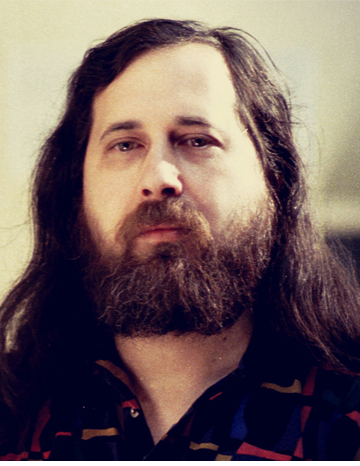
\includegraphics[width=3cm]{8_2}
\begin{center}
\footnotesize{Ричард Мэттью Столлман}
\\\footnotesize{$\mbox{род.} 1953$}
\end{center}
\end{wrapfigure}
Основоположником движения за открытый код является Ричард Мэттью Столлман. Он и создал первую лицензию GNU (General Public License).
\\Всего около 70 лицензий на владение свободным ПО (одобренных на opensource.org). Самые популярные: Apache License, BSD license, GPL, LGPL, MIT license, MPL.
\subsection{Базовые права, предоставляемые свободным ПО}
Все они предоставляют 4 базовых права:
\begin{itemize}
  \item Право на запуск программы в любых целях (только если она не нанесет вред своим действием или бездействием).
  \item Право на изучение исходного и бинарного кода программы
  \item Право на платное или бесплатное распространение программы.
  \item Право на развитие программы.
\end{itemize}
Если программист передает пользователю свою программу , но не прилагает лицензию, то действует "право свободного пользования":
\begin{itemize}
  \item Можно установить программу на 1 компьютер.
  \item Можно запускать программу на 1 компьютере.
  \item Нельзя копировать программу на другие компьютеры.
  \item Нельзя модифицировать программу.
  \item Данная лицензия действует 5 лет (п.4 ст. 1235 ГК РФ).
\end{itemize}
\subsection{Особенности различных свободных лицензий}
\begin{center}
  \textbf{GNU GPL}
\end{center}
\begin{itemize}
  \item Запрещено включать исходные тексты в закрытое ПО, запрещено менять тип лицензии (copyleft $\textcopyleft$).
  \item Запрещено динамическое связывание GNU GPL--библиотек с не--GNUGPL библиотеками (dll).
\end{itemize}
\begin{center}
  \textbf{GNU LGPL}
\end{center}
\begin{itemize}
  \item Допускается динамическое связывание с закрытыми библиотеками.
  \item Запрещено использование кода в другом ПО.
\end{itemize}
\begin{center}
  \textbf{MPL (Mozilla public license)}
\end{center}
\begin{itemize}
  \item Можно использовать исходные тексты в закрытом ПО, но
лишь частично и с гарантией доступа к изменениям.
\end{itemize}
\begin{center}
  \textbf{BSD License}
\end{center}
\begin{itemize}
  \item Можно использовать исходные коды в закрытом ПО без ограничений.
\end{itemize}
\subsection{Ответственность за пиратское ПО}
\begin{description}
  \item[Административная ответственность за пиратское ПО] Статья 7.12 КоАП РФ: нарушение авторских прав при ущербе на сумму до 100 000 рублей:
  \begin{itemize}
    \item штраф до 2 000 (физическое лицо)
    \item штраф до 20 000 (должностное лицо)
    \item штраф до 40 000 (юридическое лицо)
  \end{itemize}
  \item[Уголовная ответственность за пиратское ПО] Статья 146.2 УК РФ: незаконное использование объектов авторского права (в т.ч. приобретение, хранение) при ущербе на сумму от 100 000 рублей:
\begin{itemize}
  \item штраф до 200 000 р.
  \item исправительные работы вплоть до 2 лет
  \item – арест вплоть до 2 лет
\end{itemize}
 Статья 146.3 УК РФ: Незаконное использование объектов авторского права (в т.ч. приобретение, хранение) при ущербе на сумму от 1 000 000 рублей:
  \begin{itemize}
    \item штраф до 500 000 р.
    \item арест вплоть до 6 лет
  \end{itemize}
  \item[Уголовная ответственность за плагиат ПО] Статья 146.1 УК РФ: присвоение авторства, если это причинило крупный ущерб автору:
 \begin{itemize}
   \item штраф до 200 000 р.
   \item исправительные работы вплоть до 1 года
   \item арест вплоть до 6 месяцев
 \end{itemize}
  \item[Гражданская ответственность за нарушение лицензии ПО]  Статья 1301 ГК РФ: нарушение авторских, интеллектуальных и исключительных прав:
  \begin{itemize}
    \item штраф до 5 000 000 руб. в пользу обладателя ПО
    \\\textbf{либо}
    \item двукратное возмещение убытков обладателю ПО
  \end{itemize}
\end{description}
\section{Visual Basic for Applications}
\textbf{Visual Basic for Applications} (VBA, Visual Basic для приложений) — немного упрощенная реализация языка программирования Visual Basic, встроенная в линейку продуктов Microsoft Office (включая версии для Mac OS), а также во многие другие программные пакеты, такие как AutoCAD, SolidWorks, CorelDRAW, WordPerfect и ESRI ArcGIS. VBA покрывает и расширяет функциональность ранее использовавшихся специализированных макро--языков, таких как WordBasic.
\\
\\\textbf{Макрос} – программа, написанная на внутреннем для текстового процессора языке программирования, которую можно выполнять по желанию пользователя. Эту программу можно изменять, как и на другом языке программирования. Это позволяет автоматизировать повторяющиеся или сложные действия пользователя, которые отсутствуют в стандартном функционале текстового процессора. Таким образом можно расширять стандартный функционал.
\\
\\Использование макросов предполагает знание встроенного в текстовый процессор языка программирования. Однако современные текстовые процессоры позволяют пользователям, не знающим язык макросов, записывать свои действия для дальнейшего их преобразования в макрос. Действия пользователя автоматически описываются с помощью встроенного языка программирования. 
\\
\\Автоматической записи макроса часто бавает недостаточно, поэтому советуем ознакомиться с основами языка программирования макросов в линейке продуктов Microsoft Office Visual Basic for Applications.
\subsection{Имя переменной}
\begin{itemize}
  \item Начинается с буквы латинского алфавита.
  \item Не может содержать пробелы, точки символы операций (+, --, *, /, \#, \$, \%, \&, !, <, >, = и так далее).
  \item Не может превышать 254 символов в длину.
  \item Должно быть уникальным в своей области действия.
  \item Не может дублировать зарезервированные слова.
  \item Не различает регистр букв: MyNumber = mYnUmBeR.
\end{itemize}
\subsection{Типы данных}
\begin{minipage}{\textwidth}
\centering
\begin{tabular}{|l|c|c|c|}
\hline
Тип данных & Резервируемая & Минимальное & Максимальное \\
& память, байт & значение & значение \\
\hline
Byte & 1 & 0 & 255 \\
Boolean & 2 & False & True \\
Integer & 2 & --32768 & 32767 \\
Long & 4 & --2147483648 & 2147483647 \\
Date & 8 & 1 января 100 г. & 31 декабря 9999 г. \\
String & Длина строки & 1 & 65400 \\
Variant & \multirow{2}{*}{16} & & \\
(число) & & & \\
Variant & 22 байта + & & 2147483647 \\
(символ) & длина строки & & символов \\
\hline
\end{tabular}
\end{minipage}
\begin{center}
 \textbf{Объявление переменных}
\end{center}
\begin{enumerate}
  \item \textbf{Неявное}:
  \\sum = 100
  \\В данном случае присваивается тип Variant. Это обобщенный тип, переменная нетипизирована.
  \item \textbf{Явное}:
  \\Dim sum As Integer
  \\\emph{Преимущества}:
  \begin{itemize}
    \item Программа быстрее работает.
    \item Программе требуется меньше памяти.
    \item Легче обнаружить некоторые ошибки.
   \item Не возникает проблем со сложными типами (например, как отличить дату от текста).
  \end{itemize}
  \emph{Недостатки}:
  \begin{itemize}
    \item Приходится думать.
    \item Требуется использовать больше переменных.
  \end{itemize}
\end{enumerate}
\section{\TeX}
При взаимодействии человека с компьютером возникает вопрос: каким же образом представлять документы на экране и затем в памяти компьютера и в печатном виде. На этот счет существует 2 парадигмы:
\begin{itemize}
\item \textbf{WYSIWYG} (англ. \emph{What You See Is What You Get} -- "что видишь, то и получишь") -- свойство прикладных программ или веб--интерфейсов, в которых содержание отображается в процессе редактирования и выглядит максимально близко похожим на конечную продукцию, которая может быть печатным документом, веб--страницей или презентацией. В настоящее время для подобных программ также широко используется понятие "визуальный редактор". (пример: Microsoft Word)
\item \textbf{WYSIWYM} (англ. \emph{What You See Is What You Mean} -- "что видишь, есть то, что имеешь в виду") -- парадигма редактирования документов, возникшая как альтернатива более распространенной парадигме WYSIWYG. В WYSIWYM редакторе пользователь задает только логическую структуру документа и собственно контент. Оформление документа, его итоговый внешний вид возложено на отдельное ПО, либо, во всяком случае, вынесено в отдельный блок. Таким образом достигается полная независимость содержания документа
от его формы. (пример: \TeX)
\end{itemize}
\textbf{\TeX} -- система компьютерной верстки, разработанная американским профессором информатики Дональдом Кнутом в целях создания компьютерной типографии. В нее входят средства для секционирования документов, для работы с перекрестными ссылками. Номер версии \TeX приближается к $\pi$, номер редактора формул -- к числу $e$.
\subsection{Сравнение \LaTeX с WYSIWYG редакторами}
\LaTeX (произносится латех) — наиболее популярный набор макрорасширений (или макропакет) системы компьютерной вёрстки \TeX, который облегчает набор сложных документов. Разработан Лэсли Лэмпортом в 1984 году и назван в его честь.
\begin{table}
\begin{tabular}{|l|l|l|}
\hline
Критерий & \LaTeX & MS Word, \\
 & & LibreOffice Writer \\
\hline
 Работа& Линейное текстовое & Переключение между \\
с формулами &  представление формул & линейным и математич.  \\
 &  &  видом формулы \\
\hline
 Дизайнерские& Текстовый векторный & Встроенный векторный \\
 задачи& редактор, сложно&  WYSIWYG редактор, \\
&  управлять располо--& наглядное управление \\
&жением графики & структурой доукумента \\
\hline
Порог вхождения& Высокий& Низкий \\
\hline
Написание& Является мировым& Большинство  \\
научных статей& стандартом& российских журналов \\
\hline
Стоимость&Бесплатно&LibreOfice бесплатно \\
\hline
Рецензирование&Нет, можно&Продвинутые встроенные \\
текстов& комментировать &возможности \\
\hline
Экспорт в &\multicolumn{2}{l|}{Полноценной бесплатной утилиты для } \\
 другие форматы& \multicolumn{2}{l|}{экспорта из docx в tex и обратно не существует} \\
\hline
Требования к& Очень низкие:& \\
аппарат. обеспечению& достаточно консоли & Высокие\\
\hline
Автогенерация&Удобно генерировать& Требуется знание\\
документов&отчеты изнутри&  сложной структуры \\
 &работающих программ&  docx (odt) \\
\hline
Коллективная& &Поддерживается MSW\\
работа с файлами&Разрабатывается&  по умолчанию\\
\hline
Количество & Мало&Много \\
квалифицированных&(ученые, пользователи с& (подавляющее \\
пользователей&технич. образованием)& большинство людей) \\
\hline
Кросс--платфор--& & Большинство \\
менность ПО&Любая ОС & популярных ОС  \\
 для редактирования & &  с наличием GUI \\
\hline
Кросс--платфор--&Обратная &Проблемы при \\
менность&совместимость & обновлении версий \\
формата файла &хорошо обеспечена & \\
\hline
Проверка пунктуации&Отстутвует&Доступна по\\
и грамматики&(утилита hunspell)&умолчанию \\
\hline
Автоматизация&Отсутствует (можно& Встроенная поддержка  \\
повтор. действий &использовать скрипты) & макросов \\
\hline
Работа с & Нет ограничений&Компьютер  \\
большими файлами& & "подвисает" \\
\hline
Кодировка& На выходе получается& Проблемы из--за \\
 &PDF файл& несоответствия кодировок \\
\hline
\end{tabular}
\caption{Сравнение \LaTeX с WYSIWYG редакторами}
\end{table}
\section{Вебинары}
\textbf{Вебинар (онлайн--семинар)} -- разновидность веб--конференции, проведение онлайн--встреч или презентаций через Интернет. Во время веб--конференции каждый из участников находится у своего компьютера, а связь между ними поддерживается через Интернет посредством загружаемого приложения, установленного на компьютере каждого участника, или через веб--приложение.
\\1988 г. – появление первых IRC (англ. Internet Relay Chat).
\\Середина 1990--х – появление и распространение IM (Instant Messaging).
\\1998 г. – регистрация торгового знака "Webinar" Эриком Р. Корбом (Eric R. Korb).
\begin{center}
  Существуют следующие приложения для вебинаров
\end{center}
\begin{itemize}
  \item GoToMeeting
    \begin{itemize}
    \item Создана в 2004 году компанией Citrix Online.
    \item Поддерживаемые ОС: Macintosh, Microsoft Windows
    \item http://www.gotomeeting.com/
  \end{itemize}
  \item StartMeeting
    \begin{itemize}
    \item Создана в 2011 году как start--up.
    \item Поддерживаемые ОС: Microsoft Windows
    \item http://www.startmeeting.com/
  \end{itemize}
  \item Team Viewer
    \begin{itemize}
    \item Создана в 2005 году.
    \item Поддерживаемые ОС: Windows, Mac OS, Linux, Android, Apple iOS, Windows Phone
    \item http://www.teamviewer.com
  \end{itemize}
\end{itemize}